\section{CrN2}
\subsection*{Material ID: mp-cfvbj}
\textbf{Constante Dieléctrica ($\epsilon_{total}$):} 66.05 \\[0.5em]
\begin{table}[h!]
\centering
\begin{tabular}{lcc}
\toprule
\textbf{Métrica} & \textbf{Lámina (Plate)} & \textbf{Cilindros (Rod)} \\
\midrule
Bandgaps ($a/\lambda$) & [0.705 - 0.706], [0.722 - 0.723], [0.725 - 0.733] & Ninguno \\
Resonancias & 36 & 36 \\
\bottomrule
\end{tabular}
\end{table}
\begin{figure}[H]
\centering
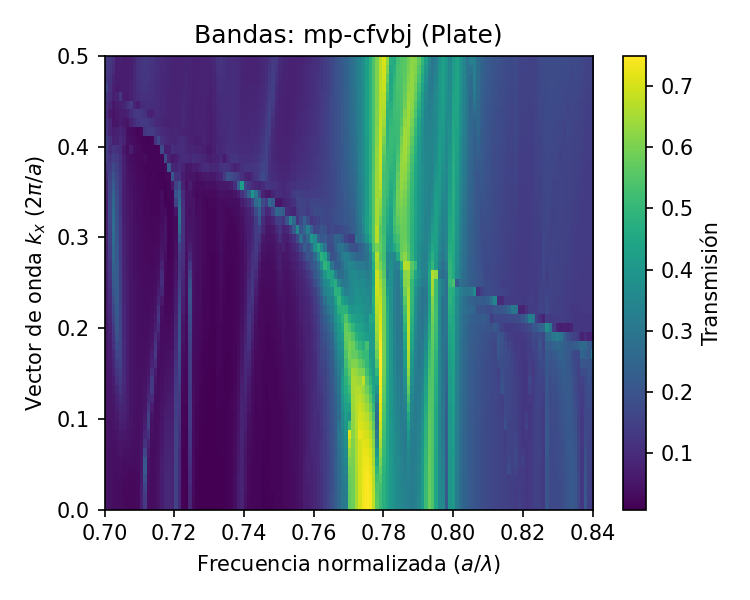
\includegraphics[width=0.48\textwidth]{figures/mp-cfvbj_plate.png}
\hfill
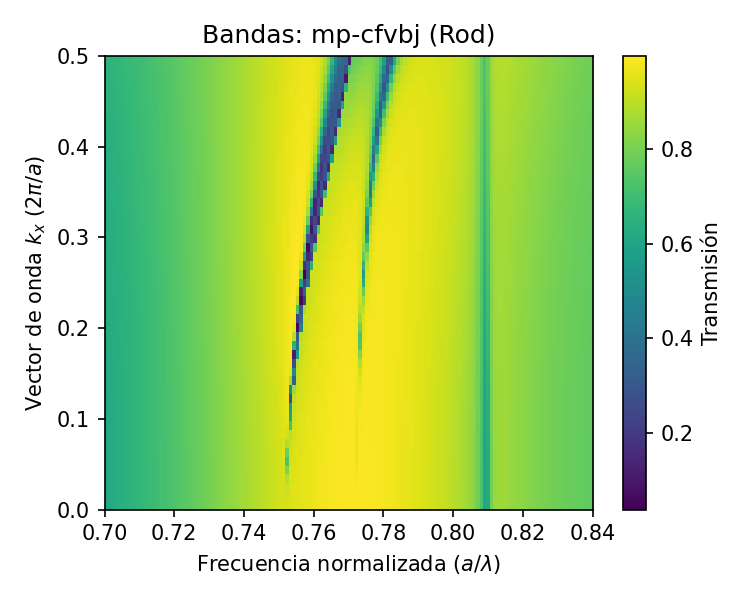
\includegraphics[width=0.48\textwidth]{figures/mp-cfvbj_rod.png}
\caption{Estructuras de bandas fotónicas para mp-cfvbj. Izquierda: Lámina. Derecha: Cilindros.}
\end{figure}
\vspace{1em}
\hrule
\vspace{1em}
\subsection*{Material ID: mp-cfvbp}
\textbf{Constante Dieléctrica ($\epsilon_{total}$):} 69.34 \\[0.5em]
\begin{table}[h!]
\centering
\begin{tabular}{lcc}
\toprule
\textbf{Métrica} & \textbf{Lámina (Plate)} & \textbf{Cilindros (Rod)} \\
\midrule
Bandgaps ($a/\lambda$) & [0.706 - 0.714] & Ninguno \\
Resonancias & 36 & 36 \\
\bottomrule
\end{tabular}
\end{table}
\begin{figure}[H]
\centering
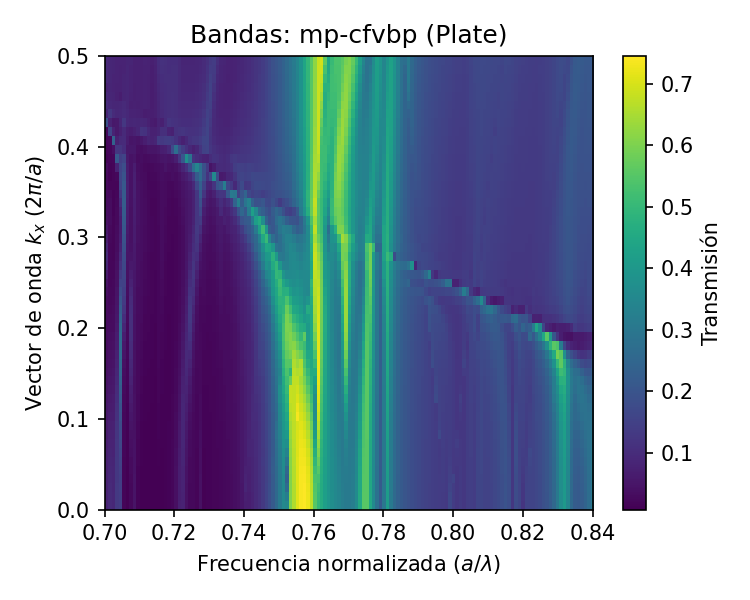
\includegraphics[width=0.48\textwidth]{figures/mp-cfvbp_plate.png}
\hfill
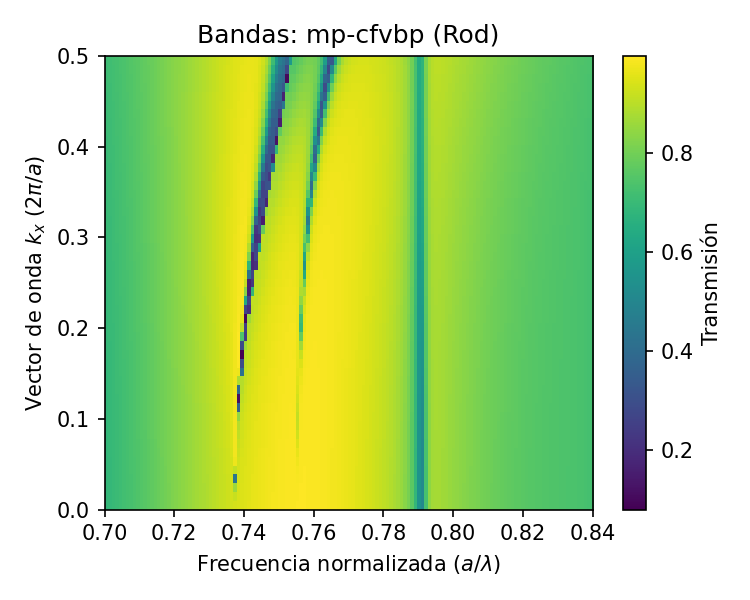
\includegraphics[width=0.48\textwidth]{figures/mp-cfvbp_rod.png}
\caption{Estructuras de bandas fotónicas para mp-cfvbp. Izquierda: Lámina. Derecha: Cilindros.}
\end{figure}
\vspace{1em}
\hrule
\vspace{1em}
\clearpage